\documentclass[A4,svgnames,9pt,aspectratio=169]{beamer}
%% document options:
%% - aspectratio = { 43, 169, 1610 }
%% - utf8
%%

%%
%% insert list of packages
%%

%% \usepackage[english,french]{babel}

\hypersetup{ 
   allcolors=bleu_utt_clair,
   pdfauthor   = {firstname lastname},
   pdftitle    = {\@title},
   pdfsubject  = {Resum\'{e} of everything},
   pdfkeywords = {firstname~lastname, curriculum vit\ae{}}
}

%%%%%%%%%%%%%%%%%%%%%%%%%%%%%%%%%%%%%%%%%%%%%%%%%%%%%%%
%%
%%%%%%%%%%%%%%%%%%%%%%%%%%%%%%%%%%%%%%%%%%%%%%%%%%%%%%%
\usepackage{blindtext}
\usepackage{appendixnumberbeamer}

\title[titrecourt]{Template Beamer UTT}
\subtitle{Pour faire des super présentation en utilisant Latek}
\date[00/00/202X]{date long}
\author[A. et al.]{Ducky le canard}
\newcommand{\semester}{A24}
\newcommand{\course}{UE name}


\usetheme{utt}

\begin{document}

% Appeler la page titre
\frame{\titlepage}

% Renommer le titre du sommaire, pour une présentation en anglais par exemple
\renewcommand{\contentsname}{Sommaire}
% Appeler la page de sommaire
%\frame{\tocpage}

%%%%%%%%%%%%%%%%%%%%%%%%%%%%%%%%%%%%%%%%%%%%%%%%%%%%%%%
\section{Utiliser Beamer}
\begin{frame}{Faire sa première slide}
    \begin{block}{exemple d'un "block", élément de base pour beamer}
       Deuxième niveau de liste (Texte courant). Ut wisi enim ad minim veniam, quis nostrud exerci tation
       ullamcorper suscipit loborti. Mauris tempor adipiscing ligula bibendum. Vestibulum sapien lectus,
       porttitor vel euismod a, lobortis at mauris.
   \end{block}

   \begin{block}{2e block}
    Deuxième niveau de liste (Texte courant). Ut wisi enim ad minim veniam, quis nostrud exerci tation
    ullamcorper suscipit loborti. Mauris tempor adipiscing ligula bibendum. Vestibulum sapien lectus,
    porttitor vel euismod a, lobortis at mauris.
\end{block}
\end{frame}

\begin{frame}{List et enumeration}
   \begin{block}{list}
      \begin{itemize}
         \item Troisième niveau de liste (Puce 1). Vestibulum sapien lectus, porttitor vel euismod a.
         \begin{itemize}
            \item Quatrième niveau de liste (Puce 2). Netus et malesuada fames ac turpis egestas.
            \item Quatrième niveau de liste (Puce 2). Netus et malesuada fames ac turpis egestas.
            \begin{itemize}
               \item Cinquième niveau de liste (Puce 2). Mauris tempor turpis eu libero sollicitudin.
               \item Cinquième niveau de liste (Puce 2). Mauris tempor turpis eu libero sollicitudin.
            \end{itemize}
          \end{itemize}
        \end{itemize}
   \end{block}

   \begin{block}{enumeration}
      \begin{enumerate}
         \item Troisième niveau de liste (Puce 1). Vestibulum sapien lectus, porttitor vel euismod a.
         \item Troisième niveau de liste (Puce 1). Vestibulum sapien lectus, porttitor vel euismod a.
         \begin{enumerate}
            \item Quatrième niveau de liste (Puce 2). Netus et malesuada fames ac turpis egestas.
            \item Quatrième niveau de liste (Puce 2). Netus et malesuada fames ac turpis egestas.
            \begin{enumerate}
               \item Cinquième niveau de liste (Puce 2). Mauris tempor turpis eu libero sollicitudin.
            \end{enumerate}
          \end{enumerate}
        \end{enumerate}
   \end{block}
\end{frame}

\begin{frame}{Tailles de polices}

   {\tiny         The quick brown fox jumps over the lazy dog}\\
   {\scriptsize   The quick brown fox jumps over the lazy dog}\\
   {\footnotesize The quick brown fox jumps over the lazy dog}\\
   {\small        The quick brown fox jumps over the lazy dog}\\
   {\normalsize   The quick brown fox jumps over the lazy dog}\\
   {\large        The quick brown fox jumps over the lazy dog}\\
   {\Large        The quick brown fox jumps over the lazy dog}\\
   {\LARGE        The quick brown fox jumps over the lazy dog}\\
   {\huge         The quick brown fox jumps over the lazy dog}\\
   {\Huge         The quick brown fox jumps over the lazy dog}

\end{frame}

\begin{frame}{Mise en page sur 2 colonnes}
   \begin{columns}
       
       \begin{column}[t]{0.45\textwidth}
           \begin{center}
           \includegraphics[width=0.95\textwidth]{imgs/photo.png}      
           \end{center}
       \end{column}
         
     \begin{column}[t]{0.45\textwidth}
 
            \begin{block}{Premier niveau de liste (Titre)}
            Deuxième niveau de liste (Texte courant).
              \begin{itemize}
                \item Troisième niveau de liste (Puce 1).
                    \begin{itemize}
                      \item Quatrième niveau de liste (Puce 2).
                         \begin{itemize}
                            \item Cinquième niveau de liste (Puce 3).
                         \end{itemize}
                    \end{itemize}
              \end{itemize}
            \end{block}
 
            \begin{block}{Premier niveau de liste (Titre)}
            Deuxième niveau de liste (Texte courant).
              \begin{itemize}
                \item Troisième niveau de liste (Puce 1).
                    \begin{itemize}
                      \item Quatrième niveau de liste (Puce 2).
                    \end{itemize}
              \end{itemize}
            \end{block}
 
          \end{column}
          
   \end{columns}
 \end{frame}


%%%%%%%%%%%%%%%%%%%%%%%%%%%%%%%%%%%%%%%%%%%%%%%%%%%%%%%

%%%%%%%%%%%%%%%%%%%%%%%%%%%%%%%%%%%%%%%%%%%%%%%%%%%%%%%
\section{Elements additionnels}
%%%%%%%%%%%%%%%%%%%%%%%%%%%%%%%%% Blocs %%%%%%%%%%%%%%
\begin{frame}
    \frametitle{Blocks spécifics}
    
    In this slide, some important text will be
    \alert{highlighted} because it's important.
    Please, don't abuse it.
    
    \begin{block}{Simple block}
    Sample text
    \end{block}
    
    \begin{theorem}{Théorème}
    Sample text in red box
    \end{theorem}
    
    \begin{examples}
    Sample text in green box. The title of the block is ``Examples".
    \end{examples}
\end{frame}

%%%%%%%%%%%%%%%%%%%%%%%%%%%%%%%%% Tableaux %%%%%%%%%%%%%%
\begin{frame}
    \frametitle{Tableaux}
    
    \begin{table}[]
        \centering
        \begin{tabular}{|c|c|c|c|}
            \hline
            UE & Semestre & Credits & Responsable  \\
            \hline
             UE 1 & A25 & 18   &  Mr. Tomate  \\
             UE 2 & P24 & 12   &  Mr. Poireau  \\
             UE 3 & A24 & 16   &  Mr. Patate  \\
             \hline
        \end{tabular}
        \caption{Exemple d'un tableau}
        \label{tab:surrogates}
    \end{table}
\end{frame}

%%%%%%%%%%%%%%%%%%%%%%%%%%%%%%%%% FIGURES %%%%%%%%%%%%%%
\begin{frame}{Figures}
    \begin{figure}
        \centering
        \includegraphics[width=0.3\textwidth]{assets/imgs/img_utt.png}
        \caption{Insertion d'une figure}
    \end{figure}  
\end{frame}
%%%%%%%%%%%%%%%%%%%%%%%%%%%%%%%%%%%%%%%%%%%%%%%%%%%%%%%

%%%%%%%%%%%%%%%%%%%%%%%%%%%%%%%%%%%%%%%%%%%%%%%%%%%%%%%
\section{Animation}
%%%%%%%%%%%%%%%%%%%%%%%%%%%%%%%%% Animation enumerate %%%%%%%%%%%%%%
\begin{frame}{Animation sur une liste (ou énumeration)}
    This is a text in second frame. 
    For the sake of showing an example.
    
    \begin{itemize}
     \item<1-> Text visible from slide 1
     \item<2-> Text visible on slide 2
     \item<3> Text visible on slide 3
     \item<4-> Text visible on slide 4
    \end{itemize}
\end{frame}

%%%%%%%%%%%%%%%%%%%%%%%%%%%%%%%%% Animation frame %%%%%%%%%%%%%%
\begin{frame}{Animation sur un enumerate}
    \begin{columns}
        \begin{column}{0.45\textwidth}

            \onslide<1,3>\begin{block}{1er block}
                Texte du premier block, visible sur la premiere et la troisième slide.
                
            \end{block}
            
        \end{column}
        \begin{column}{0.45\textwidth}
            \onslide<2>\begin{figure}
                \centering
                \includegraphics[width=0.5\textwidth]{assets/imgs/img_utt.png}
                \caption{Figure visible seulement sur la 2e}
            \end{figure}  
            
        \end{column}
    \end{columns}
\end{frame}
%%%%%%%%%%%%%%%%%%%%%%%%%%%%%%%%%%%%%%%%%%%%%%%%%%%%%%%

%%%%%%%%%%%%%%%%%%%%%%%%%%%%%%%%%%%%%%%%%%%%%%%%%%%%%%%
\section{Tikz}
%%%%%%%%%%%%%%%%%%%%%%%%%%%%%%%%% TIKZ Figure %%%%%%%%%%%%%%

\begin{frame}{ Une simple figure}
\begin{figure}
    \centering
    \begin{tikzpicture}

    \begin{tikzpicture}[scale = 2]

        \draw[] (0,0) -- (1,0) node(a2)[right] {$a_2$};
        \draw[] (1,0) -- (0.8,0.5) node(a3)[above] {$a_3$};
        \draw[] (0.8,0.5) -- (0,0) node(a1)[left] {$a_1$};
        \node [anchor = north] at (0.5, -0.1){simplex $A$};
        
        \draw[->] (1.2, 0.3) -- (2, 0.3);
        
        \draw[] (2,0) -- (3,0) node(a2b)[right] {$a_2$};
        \draw[] (3,0) -- (2.8,0.5) node(a3b)[above] {$a_3$};
        \draw[] (2.8,0.5) -- (2,0) node(a1b)[left] {$a_1$};
        
        \fill[red] (2.7,0) circle (0.03);
        \draw[red, thick] (2.8,0.5) -- (2.7,0) node(ap)[below] {$a^*$};
        
        \fill[blue!30, opacity = 0.5] (2,0) -- (2.7,0) -- (2.8,0.5);
        \fill[orange!30, opacity = 0.5] (3,0) -- (2.7,0) -- (2.8,0.5);
        
        \node[left of = a3b, anchor = west, blue ]{$A_1$};
        \node[above of = a2b, anchor = north, orange ]{$A_2$};
        
            
        \end{tikzpicture}


\end{tikzpicture}
    \caption{première figure}

\end{figure}
    
\end{frame}

%%%%%%%%%%%%%%%%%%%%%%%%%%%%%%%%%Figure animé %%%%%%%%%%%%%%

\begin{frame}{Figure animé}

    \begin{figure}
        \centering
        \input{assets/tikz_picture/simple_animate.tex}
        \caption{Figure animé}
    
    \end{figure}
    
\end{frame}

%%%%%%%%%%%%%%%%%%%%%%%%%%%%%%%%% Plots %%%%%%%%%%%%%%

\begin{frame}{Graphiques}
    \begin{columns}
        \begin{column}{0.45\textwidth}
            \begin{figure}[h]
                \centering
                \input{assets/tikz_picture/plot.tex}
                \caption{Graphique avec des fonctions}
            \end{figure}
            
        \end{column}
        \begin{column}{0.45\textwidth}
            \begin{figure}[h]
                \centering
                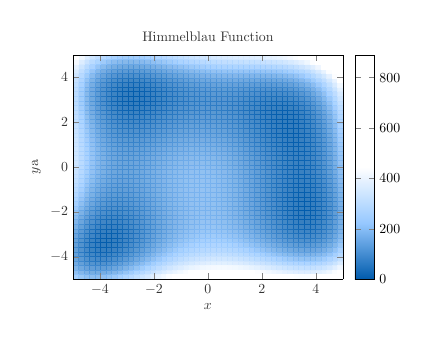
\begin{tikzpicture}[scale = 0.5]
    \begin{axis}[
        colormap={pastel}{ rgb255=(0,91,172) rgb255=(150,200,255) rgb255=(255,255,255)rgb255=(255,255,255)rgb255=(255,255,255)} ,
        view={0}{90},    % Top-down view
        enlargelimits=false,
        axis on top,
        colorbar,        % Add a colorbar
        xlabel=$x$, ylabel=$y$a,
        title={Himmelblau Function},    
        fill opacity=0.8    
    ]
    \addplot3[surf,shader=flat,z buffer=sort,samples=50,domain=-5:5] 
        { (x^2 + y - 11)^2 + (x + y^2 - 7)^2 };
    \end{axis}
\end{tikzpicture}
                \caption{Heatmap pour une fonction prenant 2 dimensions comme argument}
            \end{figure} 
            
        \end{column}
    \end{columns}
\end{frame}


%%%%%%%%%%%%%%%%%%%%%%%%%%%%%%%%%%%%%%%%%%%%%%%%%%%%%%%


%%%%%%%%%%%%%%%%%%%%%%%%%%%%%%%%%%%%%%%%%%%%%%%%%%%%%%% 
\section{Conclusion}
\begin{frame}{Conclusion}
    Une conclusion
\end{frame}


%%%%%%%%%%%%%%%%%%%%%%%%%%%%%%%%%%%%%%%%%%%%%%%%%%%%%%%
\appendix
%% Le texte est modifiable en changeant \thankyou
%% \renewcommand{\thankyou}{Thank You.}
\frame{\merci}


\begin{frame}{Annexes 1}
    Pour du contenu supplémentaire
    
\end{frame}

\begin{frame}{Annexes 2}
    Pour du contenu supplémentaire, une deuxième fois
    
\end{frame}

%%%%%%%%%%%%%%%%%%%%%%%%%%%%%%%%%%%%%%%%%%%%%%%%%%%%%%% 

\end{document}

%%%%%%%%%%%%%%%%%%%%%%%%%%%%%%%%%%%%%%%%%%%%%%%%%%%%%%%
%%
%%%%%%%%%%%%%%%%%%%%%%%%%%%%%%%%%%%%%%%%%%%%%%%%%%%%%%%

